\documentclass[10pt, letterpaper]{article}

\usepackage{amsmath}
\usepackage{enumitem}
\usepackage{float}
\usepackage{graphicx}

\setenumerate[1]{label=\thesection-\arabic*.}

\title{Solutions to The Algorithm Design Manual by Steven S. Skiena}
\author{Leo Sukharev}
\date{\today}

\begin{document}
    \maketitle
    \newpage

    \section{Introduction to Algorithm Design}

    \begin{enumerate}
        \subsection*{Finding Counterexamples}

        \item \textit{[3]} Show that $a + b$ can be less than $min(a,b)$.
        \begin{gather*}
            a = -1 \\
            b = -1 \\
            a + b = -1 + (-1) = -2 \\
            min(a,b) = min(-1, -1) = -1
        \end{gather*}

        \item \textit{[3]} Show that $a \times b$ can be less than $min(a,b)$.
        \begin{gather*}
            a = -1 \\
            b = 2 \\
            a \times b = -1 \times 2 = -2 \\
            min(a,b) = min(-1, 2) = -1
        \end{gather*}

        \item \textit{[5]} Design/draw a road network with two points $a$ and $b$ such that the
        fastest route between $a$ and $b$ is not the shortest route.

        \begin{figure}[H]
            \centering
            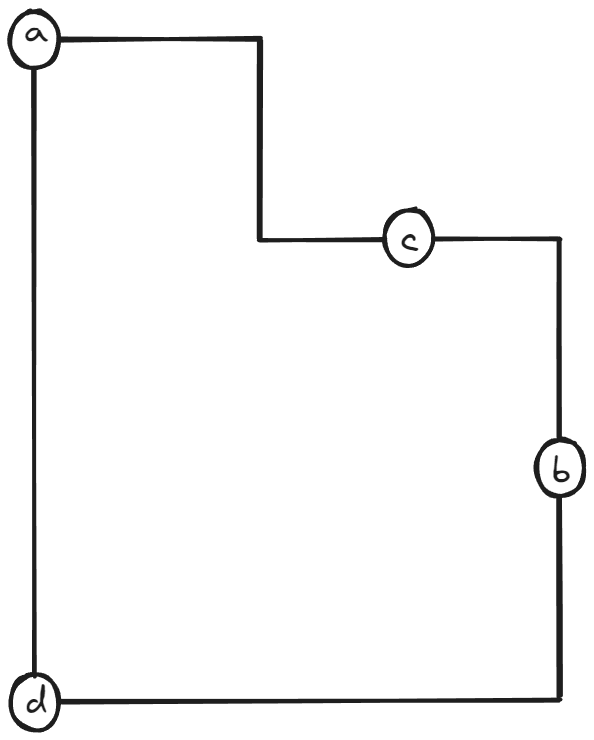
\includegraphics[scale=0.25]{01-03.png}
            \caption{Road Network}
            \label{fig:road}
        \end{figure}
        The route from $a$ to $b$ going through $c$ is shorter than the route going through $d$.
        However, the route through $c$ has more turns and a lower speed limit as a result. Since the
        route through $d$ has fewer turns and a greater speed limit, it is the fastest route from
        $a$ to $b$.

        \item \textit{[5]} Design/draw a road network with two points $a$ and $b$ such that the
        shortest route between $a$ and $b$ is not the route with the fewest turns.

        In Figure \ref{fig:road}, the route from $a$ to $b$ going through $c$ is shorter than the
        route going through $d$. The route going through $d$ has fewer turns than the route going
        through $c$.

        \item \textit{[4]} The \textit{knapsack problem} is as follows: given a set of integers
        $S = \{s_1, s_2, \ldots, s_n\}$, and a target number $T$, find a subset of $S$ that adds up
        exactly to $T$. For example, there exists a subset within $S = \{1, 2, 5, 9, 10\}$ that adds
        up to $T = 22$ but not $T = 23$.

        Find counterexamples to each of the following algorithms for the knapsack problem. That is,
        give an $S$ and $T$ where the algorithm does not find a solution that leaves the knapsack
        completely full, even though a full-knapsack solution exists.

        \begin{enumerate}
            \item Put the elements of $S$ in the knapsack in left to right order if they fit, that
            is, the first-fit algorithm.
            \begin{gather*}
                S = \{1, 2\} \\
                T = 2
            \end{gather*}

            \item Put the elements of $S$ in the knapsack from smallest to largest, that is, the
            best-fit algorithm.
            \begin{gather*}
                S = \{1, 2\} \\
                T = 2
            \end{gather*}

            \item Put the elements of $S$ in the knapsack from largest to smallest.
            \begin{gather*}
                S = \{2, 3, 4\} \\
                T = 5
            \end{gather*}
        \end{enumerate}

        \item \textit{[5]} The \textit{set cover problem} is as follows: given a set $S$ of subsets
        $S_1, \ldots, S_m$ of the universal set $U = \{1, \ldots, n\}$, find the smallest subset of
        subsets $T \subseteq S$ such that $\cup_{t_i \in T} t_i = U$. For example, consider the
        subsets $S_1 = \{1, 3, 5\}$, $S_2 = \{2, 4\}$, ${S_3 = \{1, 4\}}$, and $S_4 = \{2, 5\}$. The
        set cover of $\{1, \ldots, 5\}$ would then be $S_1$ and $S_2$.

        Find a counterexample for the following algorithm: Select the largest subset for the cover,
        and then delete all its elements from the universal set. Repeat by adding the subset
        containing the largest number of uncovered elements until all are covered.
        \begin{gather*}
            U = \{1, 2, 3, 4, 5, 6\} \\
            S_1 = \{1, 2, 3\} \\
            S_2 = \{1, 4\} \\
            S_3 = \{2, 5\} \\
            S_4 = \{3, 6\}
        \end{gather*}

        \item \textit{[5]} The \textit{maximum clique} problem in a graph $G = (V, E)$ asks for the
        largest subset $C$ of vertices $V$ such that there is an edge in $E$ between every pair of
        vertices in $C$. Find a counterexample for the following algorithm: Sort the vertices of $G$
        from highest to lowest degree. Considering the vertices in order of degree, for each vertex
        add it to the clique if it is a neighbor of all vertices currently in the clique. Repeat
        until all vertices have been considered.
        \begin{figure}[H]
            \centering
            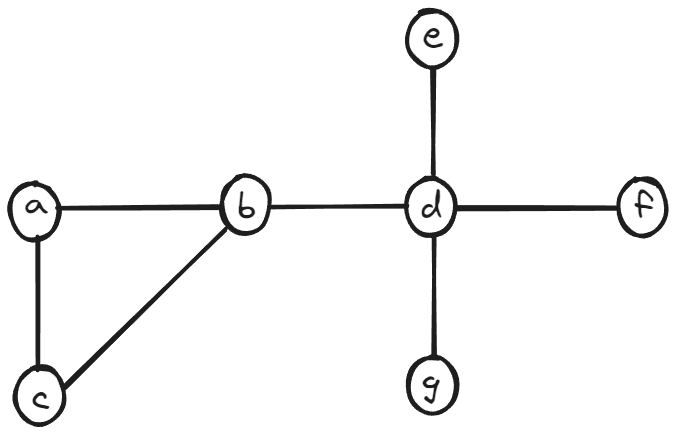
\includegraphics[scale=0.25]{01-07.png}
            \caption{Maximum Clique Counterexample}
            \label{fig:max-clique}
        \end{figure}
        Vertex $d$ has the highest degree of graph $G$, so it will be considered first. Since the
        clique is initially empty, vertex $d$ will be added to the clique. However, the maximum
        clique in Figure \ref{fig:max-clique} is $a, b, c$.
    \end{enumerate}
\end{document}
